% !TEX encoding = UTF-8
% !TEX TS-program = pdflatex
% !TEX root = ../tesi.tex

%**************************************************************
\chapter{Progettazione e codifica}
\label{cap:progettazione-codifica}
%**************************************************************

\intro{In questo capitolo vengono analizzati in modo dettagliato i moduli di \gls{backend} e \gls{frontend} del progetto Voting-Online, descrivendo per entrambi le tecnologie utilizzate, la progettazione effettuata ed illustrando infine le maschere implementate.}\\

%**************************************************************
\section{Backend}
Il progetto di stage proposto dall'azienda Sync Lab, prevedendo le prime tre settimane di formazione ed approfondimento riguardo al linguaggio Java e ai moduli fondamentali del \gls{frameworkg} Spring, mi ha permesso di realizzare, oltre al Frontend con Angular e React, anche il Backend per un consolidamento dello studio più efficace. Grazie a questa implementazione è stato possibile riutilizzare gli stessi servizi web \gls{rest} per fornire i dati a entrambi i \gls{frontend}, senza dover trovare soluzioni diverse allo stesso problema per le due tecnologie sopraccitate.

\subsection{Tecnologie}
Di seguito viene data una breve panoramica delle tecnologie utilizzate per lo sviluppo del Backend.

\subsubsection*{Maven}
\noindent In informatica Apache Maven \footcite{maven} è uno strumento di gestione di progetti software basati su Java e build automation. \\
Maven usa un costrutto conosciuto come \textit{Project Object Model} (POM); un file XML che descrive le dipendenze fra il progetto e le varie versioni di librerie necessarie nonché le dipendenze fra di esse. In questo modo si separano le librerie dalla directory di progetto utilizzando questo file descrittivo per definirne le relazioni.
\begin{figure}[h] 
    \centering 
    
\includegraphics[width=0.6\columnwidth]{immagini/cap4/Apache-maven.jpg} 
    \caption{Logo di Apache Maven}
\end{figure}
Maven effettua automaticamente il download di librerie Java e plug-in Maven dai vari repository definiti scaricandoli in locale o in un repository centralizzato lato sviluppo. Questo permette di recuperare in modo uniforme i vari file JAR e di poter spostare il progetto indipendentemente da un ambiente all'altro avendo la sicurezza di utilizzare sempre le stesse versioni delle librerie. \\
Il vantaggio derivante dall'utilizzo di questo strumento risulta molto rilevante in quanto la \textit{build automation} permette l'automatizzazione dell'intero processo di sviluppo software, il quale normalmente è composto da diverse fasi, riducendo quindi il carico di lavoro del programmatore e diminuendo le possibilità di errore da parte dello stesso.

\subsubsection*{Spring Framework}
\begin{figure}[!h] 
    \centering 
    
\includegraphics[width=0.6\columnwidth]{immagini/cap4/spring_logo.png} 
    \caption{Logo del framework Spring}
\end{figure}
\noindent In informatica Spring\footcite{spring} è un \gls{frameworkg} \gls{open-sourceg} per lo sviluppo di applicazioni su piattaforma Java, nato con l'intento di gestire la complessità nello sviluppo di applicazioni enterprise. Il \gls{frameworkg} in questione utilizza lo strumento Maven per gestire il concetto di \gls{inversion-of-controlg}, il quale è stato reso popolare negli anni proprio da Spring. \\
Il \gls{frameworkg} Spring risulta un'ottima soluzione per lo sviluppo di applicazioni Java in quanto ha diverse caratteristiche importanti a suo favore:
\begin{itemize}
    \item E' \textit{leggero} in quanto ha una struttura estremamente modulare e risulta quindi possibile utilizzare diverse funzionalità solo quando necessario, aggiungendone di nuove in modo incrementale senza sconvolgere il progetto in sviluppo;
    \item E' \textit{semplice} in quanto offre diversi moduli per una semplice risoluzione di vari problemi nello sviluppo software, come per esempio l'interfacciamento ad un Database o la gestione dell'autenticazione ed autorizzazione degli utenti nella propria applicazione;
    \item E' \textit{facile da testare} in quanto il \gls{frameworkg} nasce con la concezione che il codice di qualità debba essere facilmente testato, mettendo quindi a disposizione diversi strumenti nativi per varie tipologie di testing.
\end{itemize}

% TODO
%Descrizione degli endpoint disponibili per il frontend?

%\subsubsection*{MySQL}
%\noindent In informatica

\subsection{Descrizione}
Il \gls{backend} consiste in un servizio web \gls{rest} realizzato utilizzando il linguaggio di programmazione Java e il \gls{frameworkg} Spring. Il progetto di base, creato sulla piattaforma Spring Initializr \footcite{spring-initializr}, ha consentito di creare un'applicazione SpringBoot \footcite{spring-boot} che, utilizzando i moduli Spring Data-JPA \footcite{spring-jpa} e Data-REST \footcite{spring-rest}, permette l'accesso ai dati necessari ai \gls{frontend} attraverso appositi \gls{endpointg}. La persistenza dei dati in questione avviene attraverso l'utilizzo di un Database, gestito con il \gls{dbms} MySQL e hostato attraverso la piattaforma WAMP. La configurazione per l'interfacciamento di Spring al DB è disponibile nel file \codeword{application.properties}.

\subsection{Architettura}
Nella figura 4.3 viene raffigurato il diagramma dei package, il quale permette di visualizzare la struttura del modulo di Backend. \\
Di seguito vengono descritti i principali package:
\begin{itemize}
	\item \textbf{controller}: contiene gli \gls{endpointg} aggiuntivi e personalizzati necessari per fornire le funzionalità di sign-up e login in modo corretto. Ogni controller ha un riferimento con almeno uno strato di persistenza (repository), del quale può utilizzare i metodi offerti dal \gls{frameworkg} per l'interazione con le risorse presenti nel Database;
	\item \textbf{repository}: contiene la dichiarazione delle interfacce necessarie al modulo Spring Data-REST per fornire automaticamente tutti gli \gls{endpointg} utilizzabili per interagire con le risorse gestite dal \gls{frameworkg}. Nel caso dell'UserRepository è stata bloccata l'esportazione del metodo di salvataggio di un nuovo utente offerto da Spring, in modo da rendere disponibile una diversa versione della funzionalità tramite il controller UserController presente nel package controller;
	\item \textbf{model}: contiene le classi che rappresentano le entità gestite da Spring, che quindi corrispondono alle tabelle del Database, mentre i rispettivi campi dati corrispondono agli attributi;
	\item \textbf{dto}: contiene i Data Transfer Object, ovvero gli oggetti usati per trasferire dati tra il Backend e il Frontend. Questi oggetti vengono utilizzati quindi come contenitori di dati in modo da serializzare le informazioni inoltrate attraverso il protocollo HTTP sia in entrata che in uscita al modulo di Backend;
	\item \textbf{security}: contiene la definizione di un filtro utilizzato per effettuare una configurazione di sicurezza di base nel progetto. L'utilità del filtro consiste principalmente nel controllare la provenienza delle richieste HTTP, in modo da rispondere con le risorse richieste solo all'indirizzo corrispondente al \gls{frontend}, e nell'impostare correttamente l'header delle risposte fornite dal server. \\	
\end{itemize}
\begin{figure}[!h] 
    \centering 
    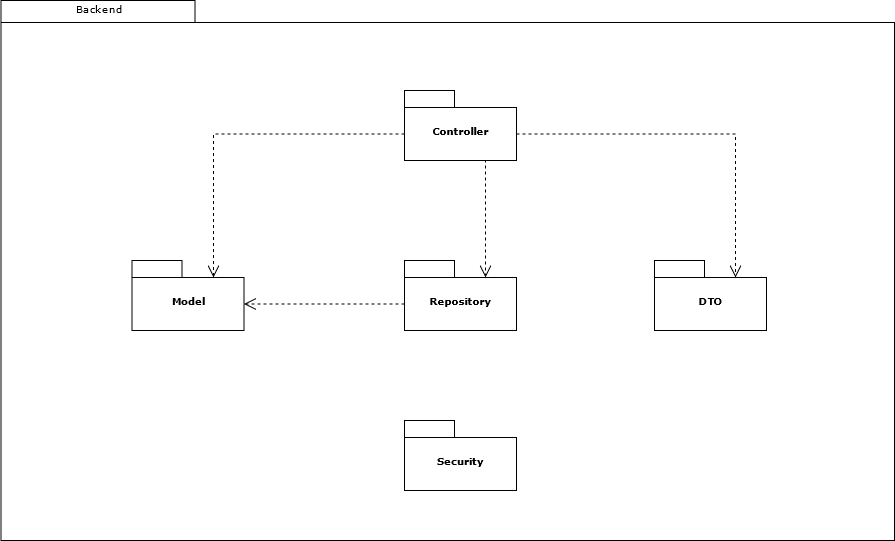
\includegraphics[width=0.9\columnwidth]{cap4/Voting-Online-BE.png} 
    \caption{Modulo Backend}
\end{figure}
%Il codice realizzato per l'implementazione del modulo in questione si trova in \href{https://github.com/killbizz/Online-Voting-BE}{questo repository} sulla piattaforma GitHub.

\subsection{Design pattern utilizzati}
\begin{itemize}
	\item \textbf{Dependency Injection}: Il dependency injection è un pattern integrato di default nel \gls{frameworkg} Spring per migliorare l'efficienza e la modularità del codice. Questo design pattern viene implementato da Spring in vari modi, in particolare nel modulo di Backend è stata utilizzata l'annotazione \textsf{Autowired} Questa annotazione consente alle classi di dichiarare tra i campi dati di quali servizi o repository si ha bisogno e in fase di inizializzazione tali dipendenze gli vengono fornite dall'esterno. Questo pattern migliora molto anche la testabilità del codice in quanto permette l'utilizzo di servizi di mock evitando di, per esempio, inviare chiamate HTTP al server vero e proprio, sostituendo dei componenti con una loro alternativa fittizia;
	\item \textbf{Singleton}\footcite{gamma:design-patterns}: Il singleton è un pattern già integrato con Spring che ha lo scopo di garantire un'unica istanza di una determinata classe in tutto l'applicativo. Il \gls{frameworkg} in questione lo implementa utilizzando l'annotazione \textsf{Bean}, la quale appunto garantisce l'esistenza di un'unica istanza della classe target e consente di iniettare quest'istanza ad ogni classe che la dichiara  come dipendenza;
\end{itemize}

% --------------------------------------------------------------------------------------------------

\section{Tecnologie per il Frontend}
Di seguito viene data una breve panoramica delle tecnologie utilizzate per lo sviluppo del Frontend. \\ \\
Per quanto riguarda \textbf{Angular}, \textbf{React} e \textbf{Next.js} viene effettuata una trattazione in modo approfondito nel \hyperref[cap:angular-react]{capitolo successivo}.

\subsubsection*{Javascript}
\begin{figure}[!h] 
    \centering 
    
\includegraphics[width=0.6\columnwidth]{immagini/cap4/Javascript_logo_2.png} 
    \caption{Logo di Javascript}
\end{figure}
\noindent \textit{JavaScript} è un linguaggio di programmazione orientato agli oggetti e agli eventi, comunemente utilizzato nella programmazione Web lato client (esteso poi anche al lato server) per la creazione, in siti web e applicazioni web, di effetti dinamici interattivi tramite funzioni di script invocate da eventi innescati a loro volta in vari modi dall'utente sulla pagina web in uso. \\
Le funzioni di script, utilizzati dunque nella logica di presentazione, possono essere opportunamente inserite in file HTML, in pagine JSP o in appositi file separati con estensione \textit{.js} poi richiamati nella logica di business. \\
Le caratteristiche principali di JavaScript sono:
\begin{itemize}
    \item essere un linguaggio interpretato;
    \item la sintassi è relativamente simile a quella dei linguaggi C;
    \item è un linguaggio debilmente tipizzato e debolmente orientato agli oggetti.
\end{itemize}
\subsubsection*{Typescript}
\begin{figure}[!h] 
    \centering 
    
\includegraphics[width=0.6\columnwidth]{immagini/cap4/Typescript_logo_2.png} 
    \caption{Logo di Typescript}
\end{figure}
\noindent \textit{TypeScript} è un linguaggio di programmazione \gls{open-sourceg} sviluppato da Microsoft e consiste in un Super-set di JavaScript che basa le sue caratteristiche su ECMAScript 6. Il linguaggio estende la sintassi di JavaScript in modo che qualunque programma scritto in JavaScript sia anche in grado di funzionare con TypeScript senza nessuna modifica. Il linguaggio  nasce dal crescente bisogno di un linguaggio frontend per lo sviluppo di applicazioni JavaScript su larga scala e dalla necessità di sicurezza e robustezza, sia da parte di sviluppatori interni a Microsoft sia da parte di clienti e sviluppatori indipendenti. Typescript è destinato ad essere compilato in JavaScript per poter essere interpretato da qualunque web browser o app. \\
Il linguaggio di programmazione in questione permette di aggiungere o rendere più flessibili e potenti varie caratteristiche di Javascript:
\begin{itemize}
    \item Firma dei metodi;
    \item Classi;
    \item Interfacce;
    \item Moduli;
    \item Operatore "=>" che permette di definire le funzioni anonime;
    \item Tipi di dato.
\end{itemize}

% ------------------------------------- ANGULAR -------------------------------------------

\section{Frontend con Angular}
\subsection{Descrizione}
Il \gls{frontend} in questione consiste in un'applicazione web realizzata con Angular, utilizzando molte delle \textit{best practices}\footcite{angular-best-practices} del \gls{frameworkg}, e il linguaggio di programmazione Typescript. \\
Il progetto di base, creato utilizzando lo strumento \codeword{ng} della Angular CLI\footcite{angular-cli}, ha permesso di sviluppare una piattaforma che fornisce agli utenti elettori ed amministratori tutte le funzionalità necessarie a soddisfare i requisiti rilevati nell'\hyperref[cap:analisi-requisiti]{analisi dei requisiti}, utilizzando i dati forniti dal \gls{backend} descritto nella precedente sezione. \\
Infine è necessario citare il fatto che il progetto Voting-Online, non avendo come focus principale la sicurezza nello sviluppo della piattaforma, ha consentito di implementatare una gestione della sessione utente utilizzando il \gls{localstorageg}, in modo da poter archiviare e recuperare semplicemente diverse informazioni ed utilizzarle per il corretto rendering lato client delle pagine web.

\subsection{Architettura di Angular}
%Angular è una framework per la creazione di applicazioni web utilizzando utilizzando di base il \hyperref[sec:site-rendering]{Client-Side Rendering}. \\
L'architettura di un'applicazione Angular si basa su alcuni concetti fondamentali. L'elemento costitutivo di base è il \textbf{component}, ovvero una classe che si occupa di gestire la vista, logica, e stile di un'intera pagina o di una determinata porzione di \gls{gui}, come descritto in modo più dettagliato nel capitolo successivo. Ogni component può a sua volta contenere diversi component figli, avendo in questo modo la possibilità di creare maschere in modo modulare ed altamente manutenibile. \\
Altri elementi fondamentali del \gls{frameworkg} in questione risultano i \textbf{servizi}, ovvero delle classi che forniscono delle funzionalità non direttamente collegate alle viste e possono essere iniettati nei component come dipendenze, e i \textbf{moduli}, i quali consistono in una collezione di servizi e configurazioni dedicate ad uno o più componenti. \\
Un'applicazione Angular è definita da un insieme di moduli ed ha sempre almeno un modulo radice che abilita il bootstrap e in genere ha molti più moduli di funzionalità.

\subsection{Architettura dell'applicazione sviluppata}
Nella figura 4.6 viene raffigurato il diagramma dei package del modulo di \gls{frontend}, il quale permette di visualizzare la struttura del progetto e contiene i seguenti  elementi fondamentali:
\begin{itemize}
	\item \textbf{components}: contiene tutti i component usati per lo sviluppo dell'applicazione, sia quelli \textit{<<principali>>}, scanditi nel file di configurazione delle rotte \textsl{routing.module.ts} e utilizzati per renderizzare intere pagine web, sia quelli \textit{<<secondari>>}, utilizzati per renderizzare delle sezioni di pagina e contenuti in quelli principali;
	\item \textbf{services}: contiene delle classi corrispondenti ai servizi Angular, i quali in particolare effettuano le chiamate HTTP al \gls{backend}, fornendo l'accesso ai dati necessari ai component;
	\item \textbf{lib}: contiene le funzioni di supporto per standardizzare le chiamate al \gls{backend};
	\item \textbf{classes}: contiene i tipi utilizzati dai component e dai service;
	\item \textbf{assets}: contiene file come immagini ed icone, utilizzate dalle viste.
\end{itemize}
\begin{figure}[!h] 
    \centering 
    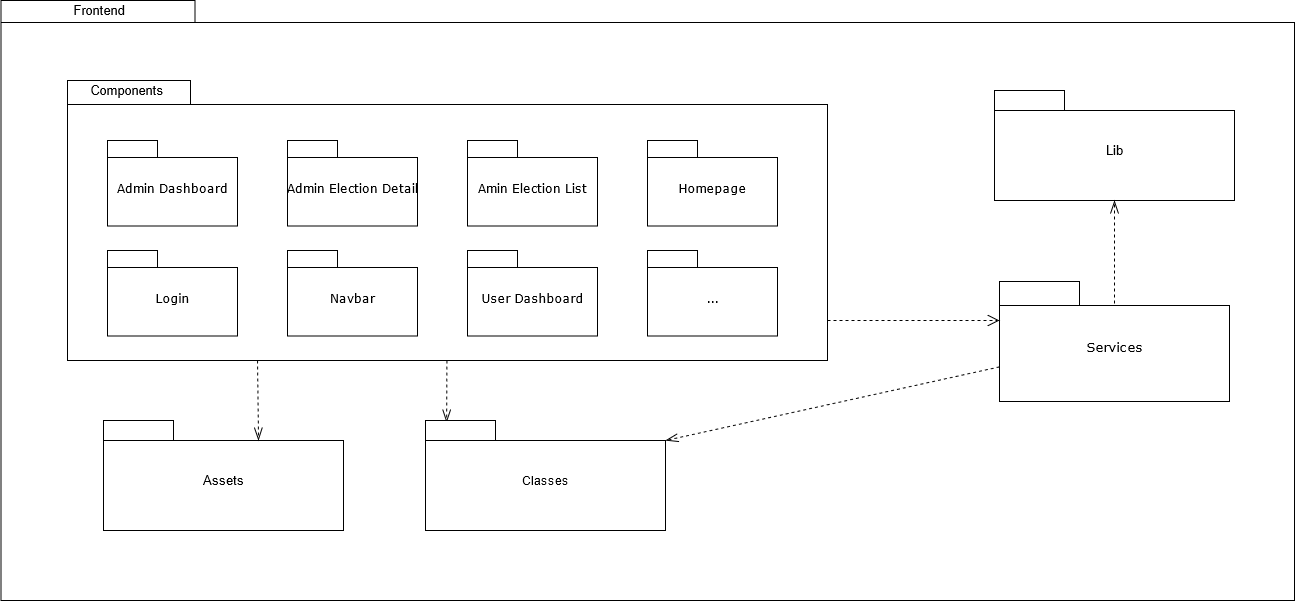
\includegraphics[width=0.9\columnwidth]{cap4/package_frontend_angular.png} 
    \caption{Modulo Frontend realizzato con Angular}
\end{figure}
\subsection{Design pattern utilizzati}
\begin{itemize}
	\item \textbf{Dependency Injection}: consiste in un design pattern per il quale è sufficiente dichiarare le dipendenze di cui un componente necessita e, quando il componente verrà istanziato, un iniettore si prenderà carico di risolvere le dipendenze (attuando dunque l'inversione del controllo). Il pattern in questione implementato da Angular è di tipo \textsf{constructor}, ovvero prevede che in ogni componente vengano dichiarati nel costruttore di quali servizi ha bisogno e in fase di inizializzazione tali dipendenze gli vengono fornite dall'esterno;
	\item \textbf{Singleton}\footcite{gamma:design-patterns}: Il singleton è un pattern integrato di default in Angular che ha lo scopo di garantire un'unica istanza di una determinata classe in tutto l'applicativo. Il \gls{frameworkg} in questione lo implementa nei \textsf{servizi}, i quali possono venire iniettati come unica istanza in diversi componenti, permettendo di condividere funzionalità e stato;
	\item \textbf{Decorator}\footcite{gamma:design-patterns}: Il decorator è un design pattern integrato di default in Angular, utile per estendere la funzionalità degli oggetti mantenendo intatte le funzionalità base degli stessi. Questo pattern è implementato in Angular come \textsf{class decorator} per indicare se una classe è di tipo component o module oppure come \textsf{property decorator} per indicare se una variabile è visibile all'esterno della classe in input o output, il tutto senza senza dover scrivere codice aggiuntivo.
\end{itemize}

% ------------------------------------- REACT -------------------------------------------

\section{Frontend con React}
\subsection{Descrizione}
Il \gls{frontend} in questione consiste in un'applicazione web realizzata utilizzando la libreria \textbf{React} per la creazione delle interfacce utente ed il \gls{frameworkg} \textbf{Next.js} per la gestione del rendering del sito. \\
Il progetto di base, creato utilizzando lo strumento \codeword{create-next-app} del package manager NPM\footcite{npm}, ha consentito lo sviluppo di una piattaforma che, allo stesso modo dell'applicazione sviluppata con Angular, fornisce agli utenti elettori ed amministratori tutte le funzionalità necessarie a soddisfare i requisiti rilevati nell'\hyperref[cap:analisi-requisiti]{analisi dei requisiti}, sfruttando i dati forniti dal \gls{backend} descritto precedentemente. \\
Infine è necessario citare il fatto che il progetto Voting-Online, non avendo come focus principale la sicurezza nello sviluppo della piattaforma, ha consentito di implementatare una gestione della sessione utente utilizzando i \gls{cookieg}, in modo da poter archiviare e recuperare semplicemente diverse informazioni ed utilizzarle per il corretto rendering lato server delle pagine web.

\subsection{Architettura dell'applicazione sviluppata}
Nella figura 4.7 viene raffigurato il diagramma dei package del modulo di \gls{frontend}, il quale permette di avere una chiara visione della struttura del progetto creato seguendo il tutorial ufficiale\footcite{next-tutorial} del \gls{frameworkg} \textit{Next.js}. Gli elementi fondamentali nell'architettura sono i seguenti:
\begin{itemize}
	\item \textbf{pages}: Next.js utilizza un sistema di routing basato sul file system, quindi i componenti React contenuti nei file dentro alla cartella pages renderizzano le pagine web presenti nella piattaforma;
	\item \textbf{components}: contiene tutti i componenti React utilizzati dalle pages per renderizzare parti della \gls{gui} dell'applicativo;
	\item \textbf{images}: contiene tutte le immagini utilizzate dalle viste;
	\item \textbf{services}: contiene tutte le funzioni che consentono di effettuare le chiamate HTTP al \gls{backend} e che forniscono i dati necessari ai component e alle pages;
	\item \textbf{classes}: contiene i tipi utilizzati dai component e dai service;
	\item \textbf{styles}: contiene l'unico file style.css, il quale applica lo stile alla piattaforma con scope globale;
	\item \textbf{lib}: contiene le funzioni di supporto utilizzate dai service per standardizzare le chiamate al \gls{backend}.
\end{itemize}
\begin{figure}[!h] 
    \centering 
    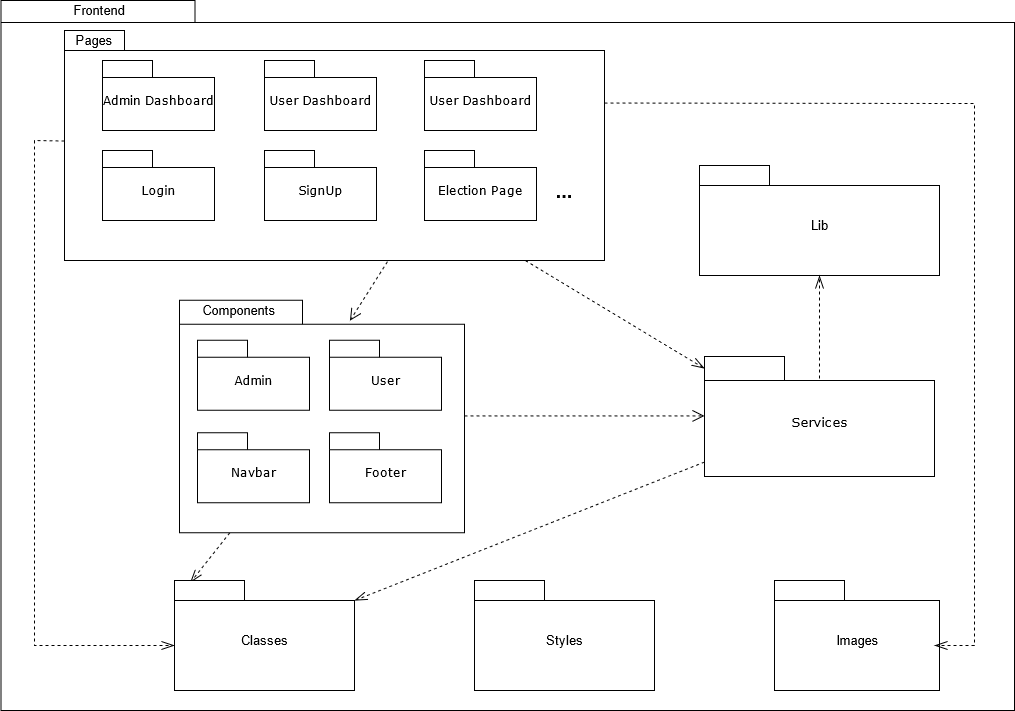
\includegraphics[width=0.9\columnwidth]{cap4/package_frontend_react.png} 
    \caption{Modulo Frontend realizzato con Next.js e React}
\end{figure}

\subsection{Il pre-rendering di Next.js}
La piattaforma, utilizzando Next.js, effettua il \hyperref[sec:site-rendering]{pre-rendering} delle pagine web lato server, ovvero genera e fornisce direttamente codice HTML, senza farlo generare al browser client. Ad ogni pagina HTML generata viene associato il codice JavaScript minimo necessario. Successivamente, quando una pagina viene caricata dal browser, il suo codice JavaScript viene eseguito e rende la pagina completamente interattiva. Nella figura 4.8 viene raffigurato uno schema generale per mostrare l'interazione tra diversi elementi del modulo in questione, in relazione al pre-rendering effettuato dalla piattaforma.
\begin{figure}[!h] 
    \centering 
    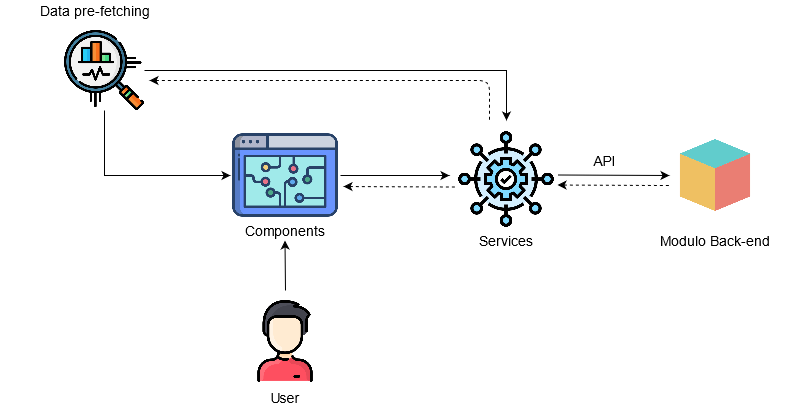
\includegraphics[width=0.9\columnwidth]{cap4/general_frontend_react.png} 
    \caption{Schema generale del Frontend in Next.js e React}
\end{figure} \\
Il \gls{frontend} utilizza il \textbf{Server-Side Rendering} (SSR), attraverso la funzione \\ \codeword{getServerSideProps} per effettuare il fetch dei dati dal \gls{backend}, nelle pagine in cui è importante avere i dati sempre aggiornati, come per esempio le dashboard dell'admin e dell'utente. \\
Viene invece utilizzato lo \textbf{Static-Site Generation} (SSG) nelle pagine in cui o non serve effettuare il fetch di dati o non è importante averli aggiornati ad ogni richiesta, come per esempio la homepage o la maschera di login. \\ \\
\textbf{NB}: Next.js effettua solamente il SSR in ambiente di sviluppo, mentre effettua anche il SSG una volta effettuato il deploy dell'applicativo.

\subsection{Design pattern utilizzati}
\begin{itemize}
	\item \textbf{React Best Practices}: le buone pratiche di React, consigliate nel sito ufficiale\footcite{react-best-practices} della libreria e dalla community, sono svariate e consentono di creare interfacce utente con codice corretto, leggibile, modulare e manutenibile. Le best practices utilizzate in particolare nel progetto in questione sono le seguenti:
	\begin{itemize}
		\item scomporre la \gls{gui} in una \textsf{gerarchia di component}, seguendo il principio di singola responsabilità tipico della programmazione ad oggetti;
		\item identificare lo \textsf{stato minimo indispensabile} necessario per ottenere tutte le funzionalità desiderate e decidere in quale component farlo giacere. Il principio base, valido in generale per qualsiasi ambito della programmazione, consiste nel DRY (ovvero <<Don't Repeat Yourself>>);
		\item utilizzare la \textsf{destrutturazione degli oggetti}, soprattutto nel caso di quelli passati tramite props, in modo da rendere il codice più snello e leggibile;
		\item utilizzare i \textsf{functional component} e i \textsf{react hooks} in quanto consentono una gestione più rapida e leggibile dello stato rispetto ai class component, anche se dal punto di vista di React le due tipologie di component sono equivalenti.
	\end{itemize}
\end{itemize}

%**************************************************************

\section{Maschere prodotte}

Con lo scopo di effettuare un paragone dettagliato tra Angular e React le maschere \gls{frontend} sono state realizzate in modo che fossero il più possibile coincidenti. Per questo motivo nell'attuale sezione, essendo le interfacce utente praticamente uguali sia a livello di funzionalità che di stile, viene elencato un unico insieme di maschere per illustrare il prodotto software, risultato del progetto in questione. Le maschere prodotte hanno permesso di soddisfare la totalità dei requisiti riscontrati nell'\hyperref[cap:analisi-requisiti]{analisi dei requisiti} per entrambe le tecnologie sopraccitate, arrivando ad avere un funzionamento completo della piattaforma che verrà descritta in seguito. \\ \\
Inoltre, prima di elencare le diverse maschere del sito, risulta utile notare la presenza in ogni pagina di una \textbf{navigation bar} dinamica in base alla tipologia di utente autenticato nella parte superiore dell'ipertesto: infatti se l'utente risulta loggato con delle credenziali da elettore ha la possibilità di accedere, tramite l'apposito link, alla dashboard personale per esprimere il proprio voto in un'elezione disponibile o visualizzare lo storico dei propri voti, oltre a visualizzare il proprio username che conferma l'esito positivo alla procedura di autenticazione. Se l'utente risulta invece autenticato come amministratore può accedere alla dashboard per la gestione delle elezioni e dei partiti nella piattaforma. In entrambi i casi è comunque disponibile un pulsante per effettuare il logout dalla piattaforma. \\
Infine è possibile notare un \textbf{footer} comune nella parte inferiore di ogni pagina dell'applicazione web.

\subsection{Homepage}
La pagina di benvenuto nella piattaforma è costituita da:
\begin{itemize}
    \item un contenuto statico per accogliere l'utente con una breve spiegazione delle funzionalità disponibili nell'applicazione;
    \item due pulsanti per indirizzare l'utente alle pagine di autenticazione o di registrazione, visualizzabili solamente dall'utente non autenticato.
\end{itemize}
\begin{figure}[H] 
    \centering 
    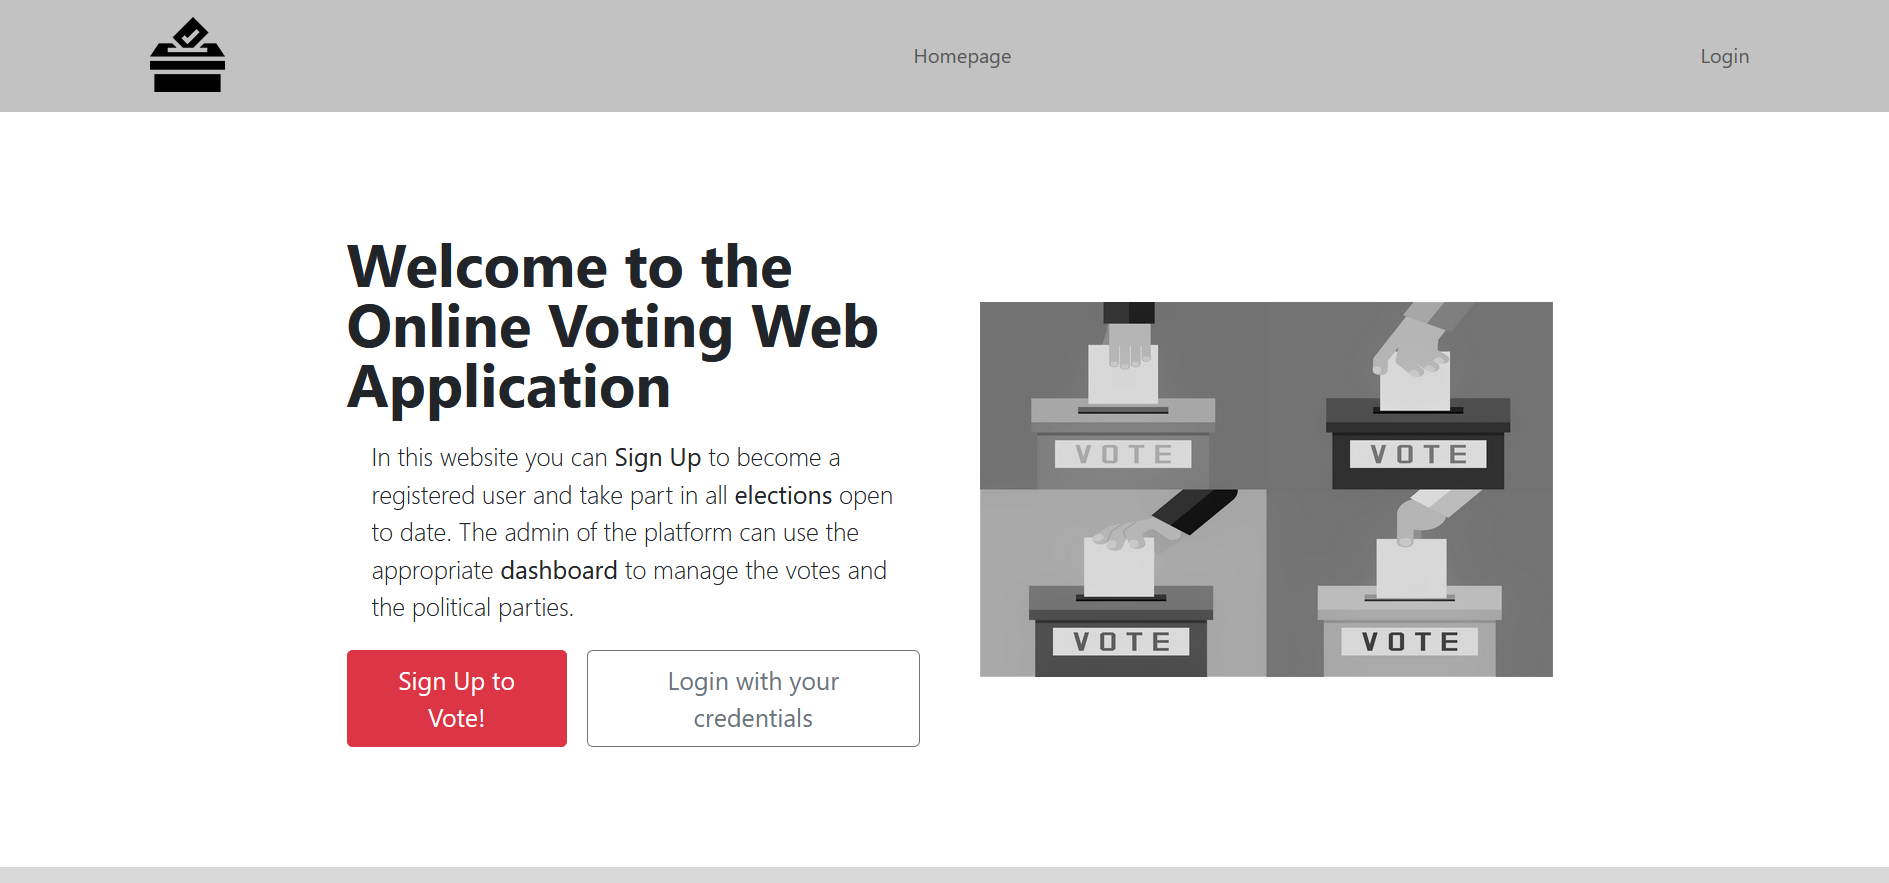
\includegraphics[width=0.8\columnwidth]{cap4/screen/home.png}
    \caption{Homepage}
\end{figure}

\subsection{Autenticazione}
La pagina di autenticazione richiede che l'utente non autenticato inserisca l' indirizzo email e la password che ha utilizzato per registrarsi nella piattaforma per poterci accedere.
\begin{figure}[H] 
    \centering 
    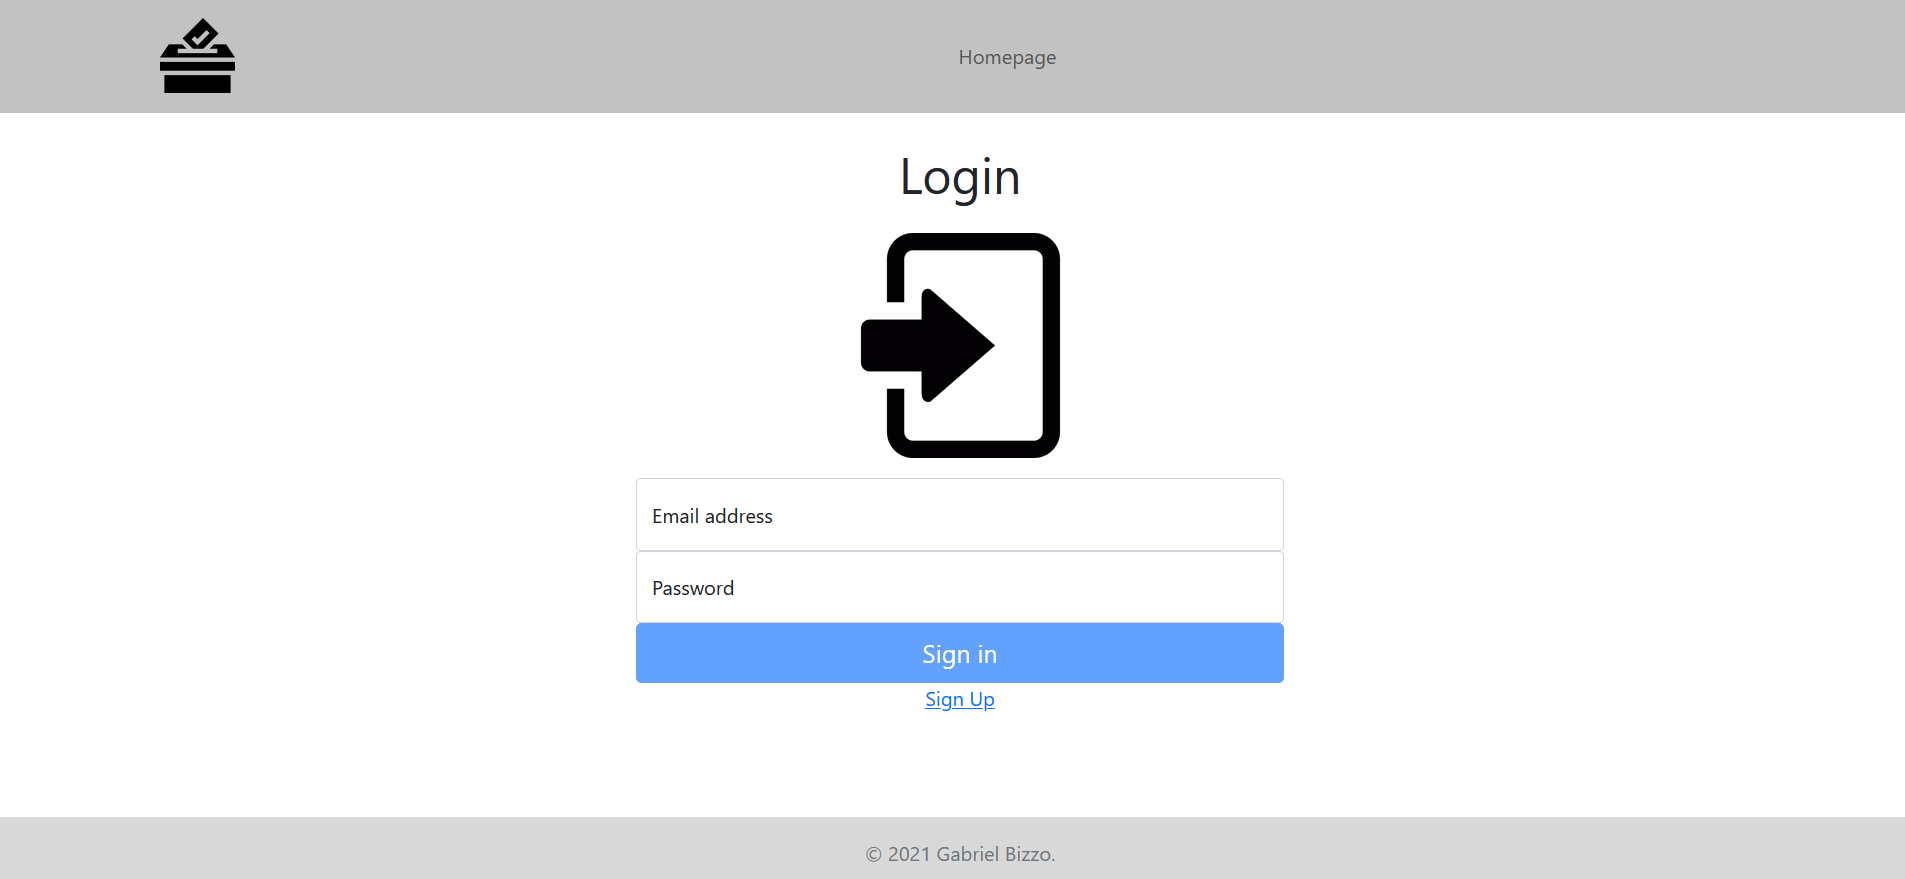
\includegraphics[width=0.75\columnwidth]{cap4/screen/login.png} 
    \caption{Pagina di autenticazione}
\end{figure}

\subsection{Registrazione}
La pagina di registrazione richiede che l'utente non autenticato inserisca l'indirizzo email, l'username e la password che desidera utilizzare all'interno della piattaforma.
\begin{figure}[H] 
    \centering 
    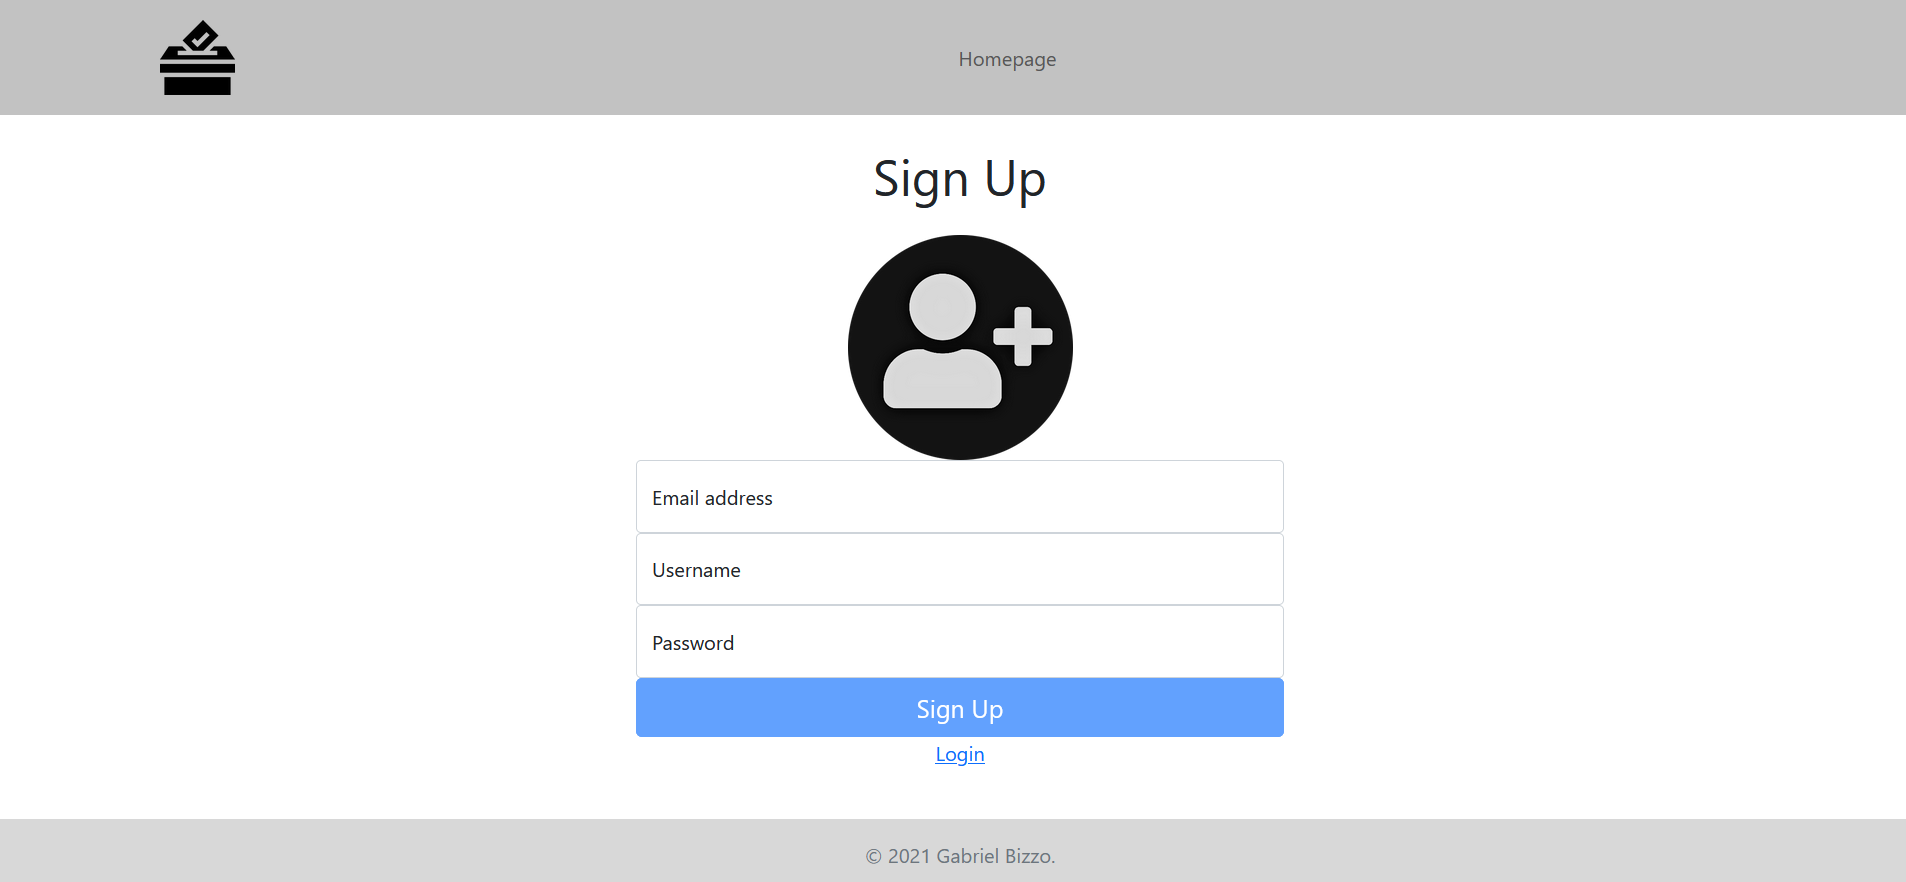
\includegraphics[width=0.75\columnwidth]{cap4/screen/sign-up.png} 
    \caption{Pagina di Registrazione}
\end{figure}

\subsection{Admin Dashboard}
L'amministratore, dopo aver effettuato la procedura di autenticazione nel sistema, può accedere alla pagina di monitoraggio della piattaforma che gli permette di gestire tutte le elezioni e i partiti in essa presenti.
\begin{figure}[H] 
    \centering 
    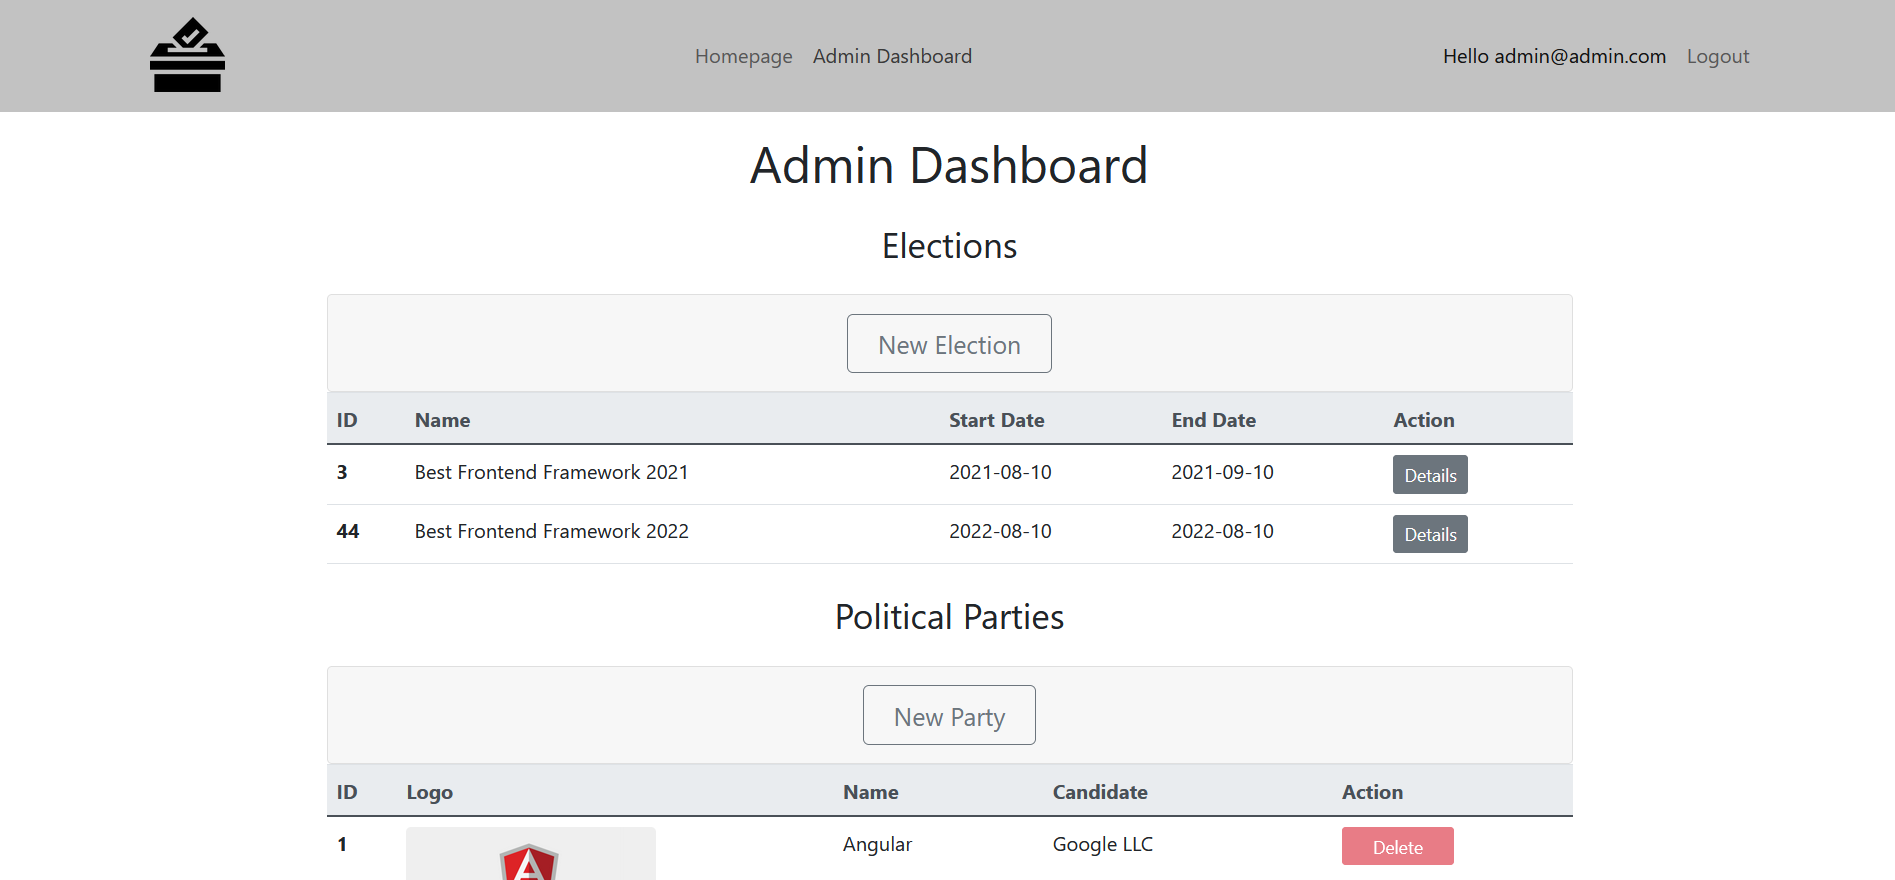
\includegraphics[width=0.75\columnwidth]{cap4/screen/admin-dash.png} 
    \caption{Pagina della Admin Dashboard}
\end{figure}

\subsubsection{Elezioni}
L'amministratore può visualizzare le informazioni di ogni elezione presente nella piattaforma nell'apposita tabella e ha la possibilità di eseguire diverse operazioni:
\begin{itemize}
    \item \textit{visualizzare i dettagli} di una singola elezione cliccando sul pulsante "Details", facendo cosi comparire una finestra in sovrimpressione che elenca il nome, la tipologia, la data di inizio e fine ed i partiti partecipanti dell'elezione desiderata;
    \item \textit{eliminare} l'elezione della quale si stanno visualizzando i dettagli cliccando sull'apposito pulsante, il quale risulta abilitato solo nel caso in cui l'elezione non risulti già cominciata o terminata;
    \item \textit{modificare} i dati dell'elezione della quale si stanno visualizzando i dettagli cliccando sull'apposito pulsante per rendere editabili i campi contenenti le informazioni. Il bottone che abilita la modifica risulta abilitato e permette l'operazione in questione solamente nel caso in cui l'elezione risulta ancora da cominciare.
\end{itemize}
\begin{figure}[H] 
    \centering 
    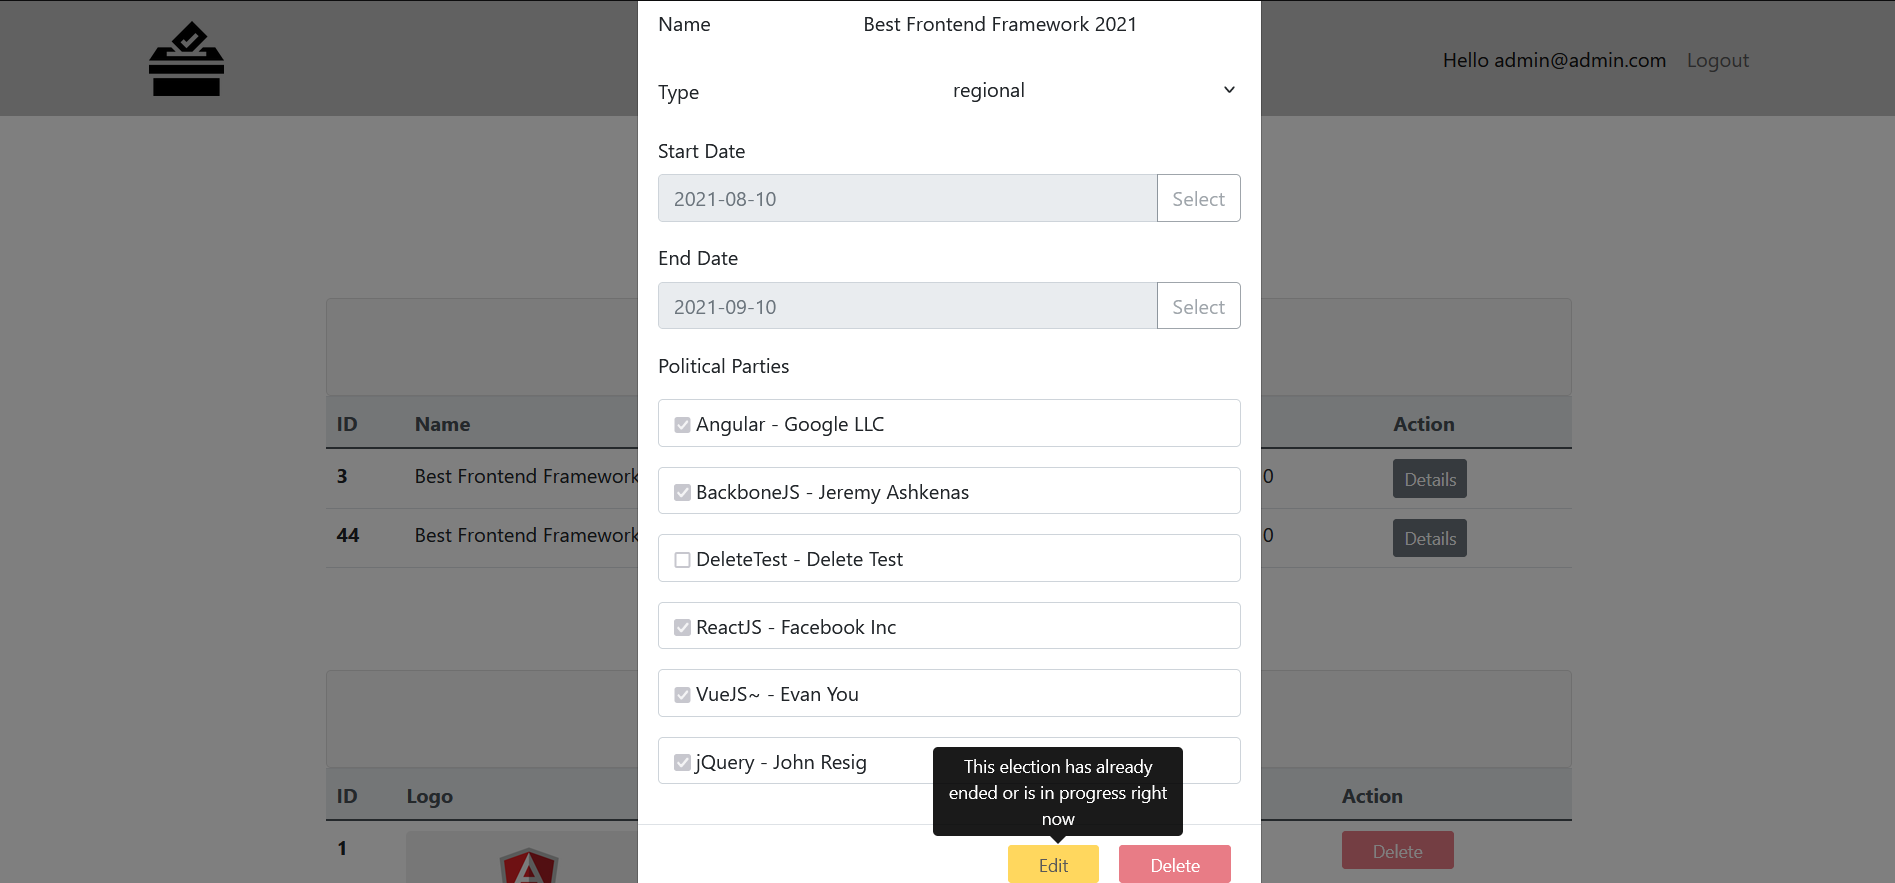
\includegraphics[width=0.75\columnwidth]{cap4/screen/admin-election-detail.png} 
    \caption{Finestra contenente i dettagli di un'elezione}
\end{figure}
L'amministratore ha la possibilità, inoltre, di \textit{aggiungere} una nuova elezione nella piattaforma compilando il form che compare cliccando il pulsante "New Election". I campi da compilare consistono nel nome, tipologia, data di inizio, data di fine ed elenco dei partiti partecipanti. Nel caso in cui i campi vengano lasciati vuoti o compilati in modo errato degli appositi messaggi verranno visualizzati in modo da consentire, in seguito ad una modifica dei campi compilati erroneamente, un ulteriore tentativo di inserimento all'utente.
\begin{figure}[H] 
    \centering 
    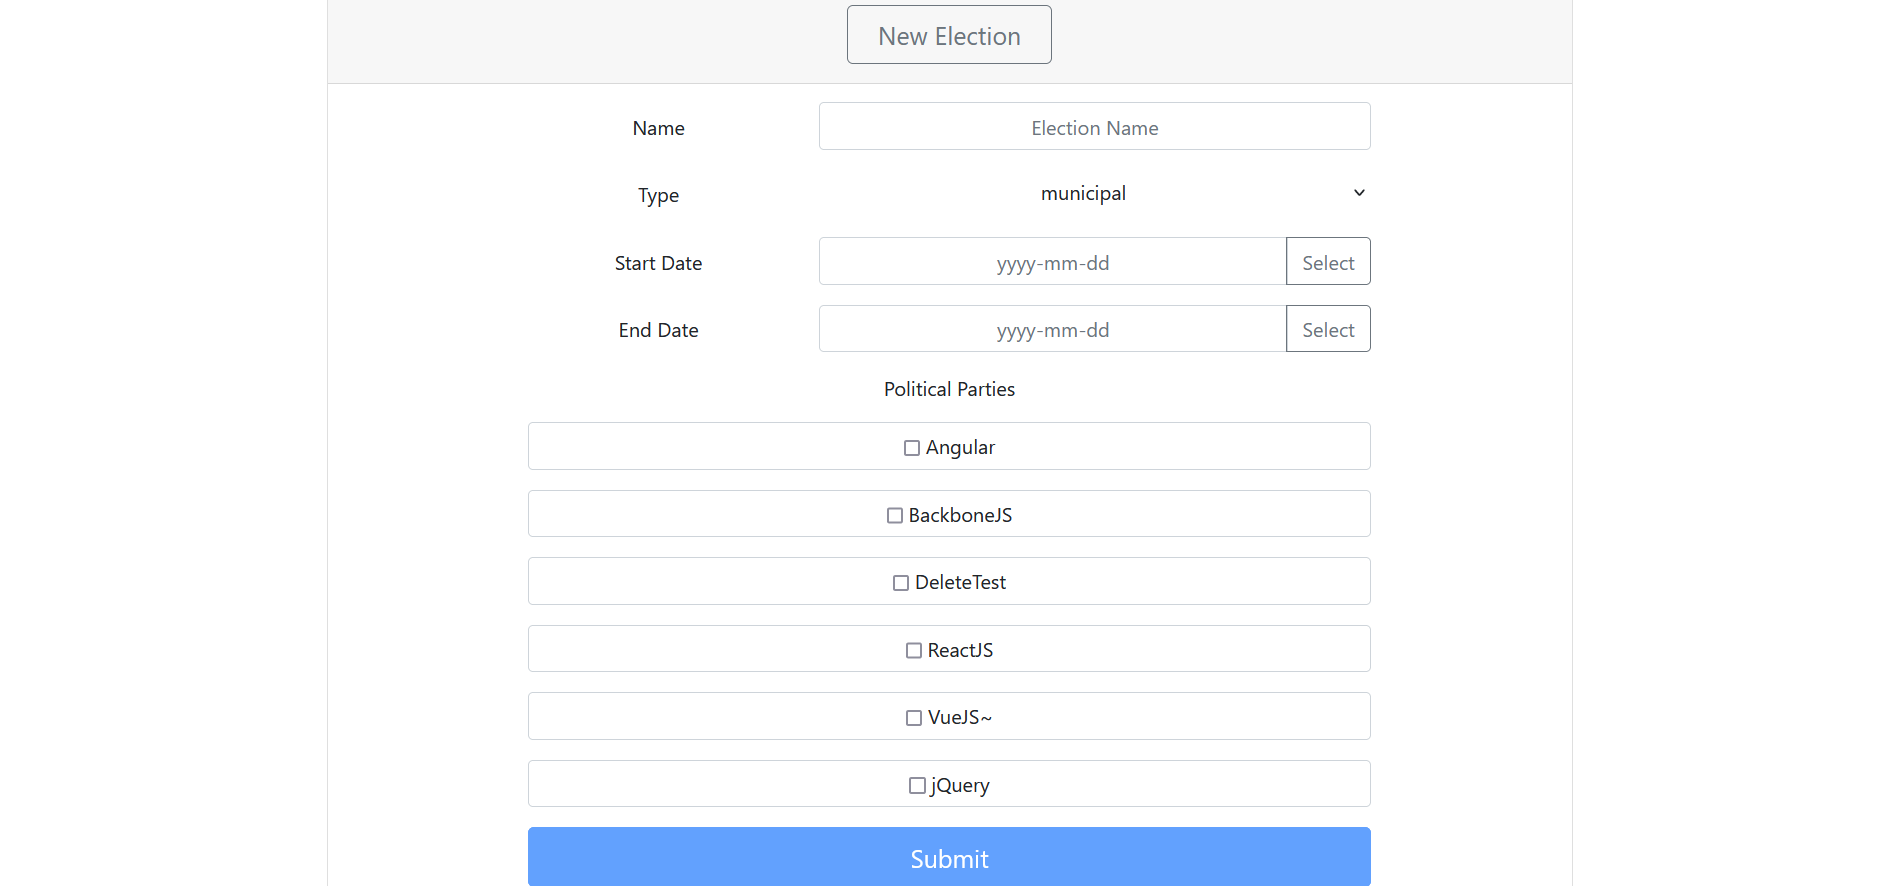
\includegraphics[width=0.75\columnwidth]{cap4/screen/new-election.png} 
    \caption{Form di creazione di una nuova elezione}
\end{figure}

\subsubsection{Partiti}
L'amministratore, in modo simile alle elezioni, ha la possibilità di effettuare diverse operazioni per la gestione dei partiti presenti nella piattaforma:
\begin{itemize}
    \item \textit{visualizzare le informazioni} di ogni partito nell'apposita tabella, in particolare il nome, logo e nominativo del candidato del partito;
    \item \textit{eliminare} un partito dalla piattaforma cliccando sull'apposito pulsante, il quale risulta abilitato solo nel caso in cui il partito non risulti già presente in un'elezione;
    \item \textit{aggiungere} un nuovo partito nella piattaforma compilando il form che compare cliccando sul pulsante "New Party". Il funzionamento del form risulta uguale a quello per creare una nuova elezione, tuttavia i campi richiesti in questo caso sono il nome, logo e nominativo del candidato del partito.
\end{itemize}

\subsection{User Dashboard}
L'elettore, dopo aver effettuato la procedura di autenticazione nel sistema, può accedere alla dashboard personale che gli permette di esprimere la propria preferenza in un'elezione disponibile e di controllare il proprio storico dei voti.
\begin{figure}[H] 
    \centering 
    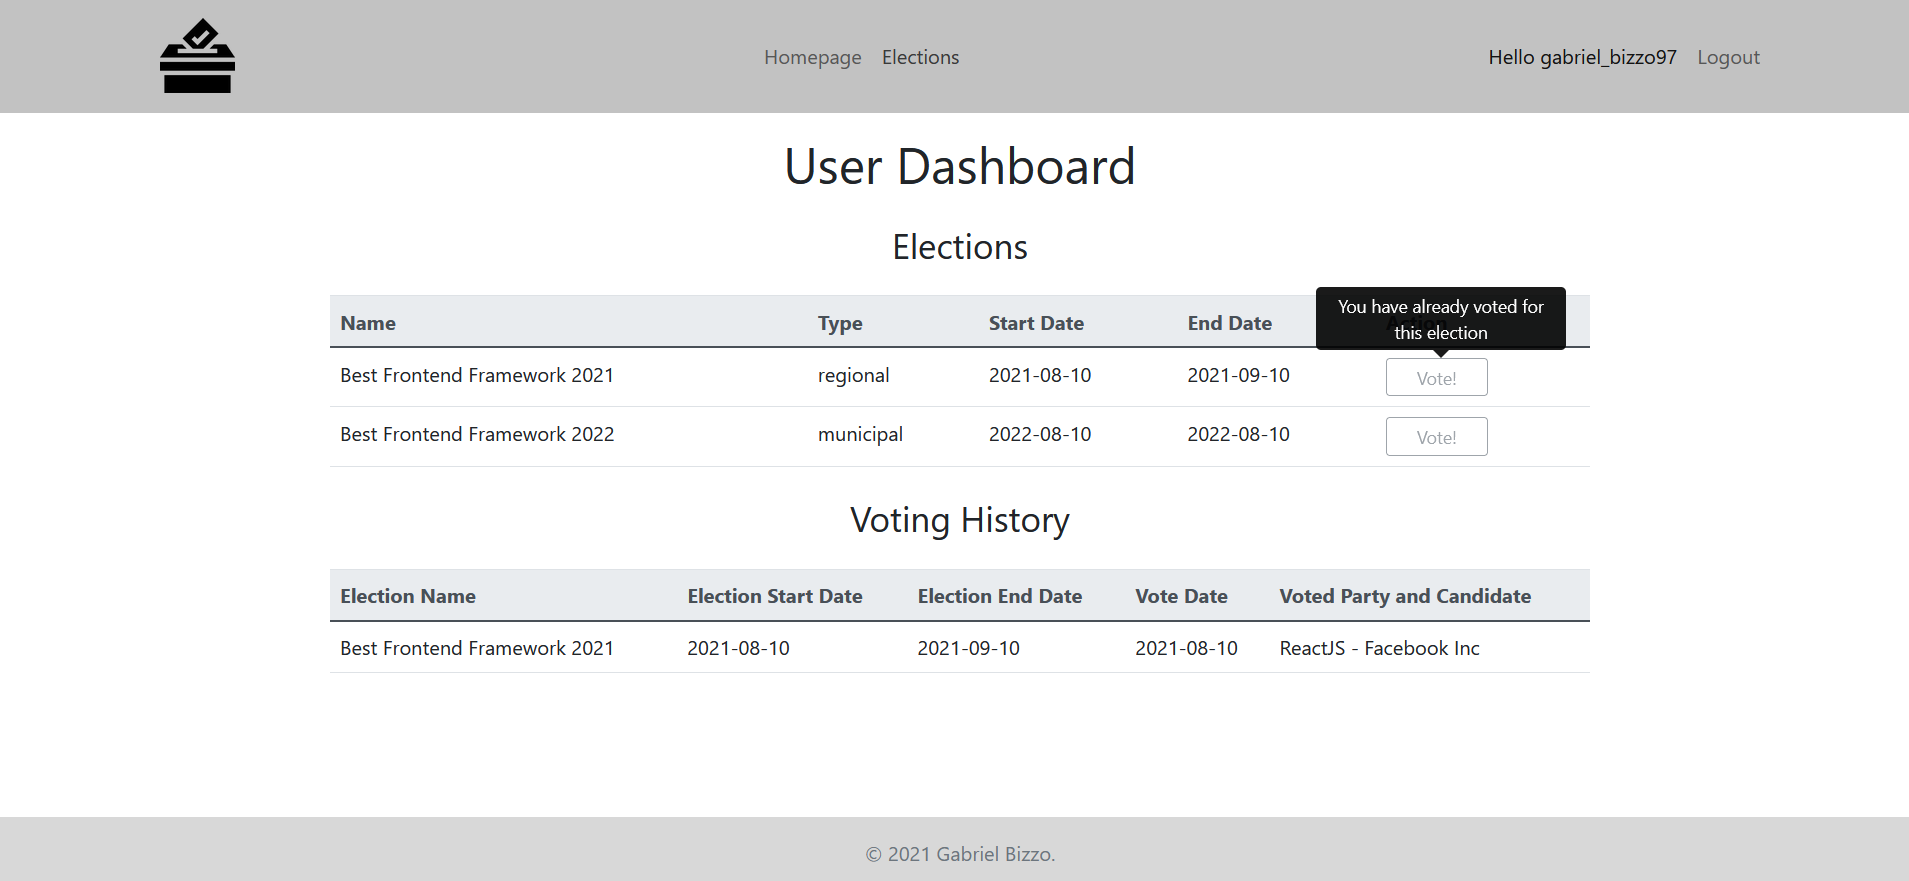
\includegraphics[width=0.75\columnwidth]{cap4/screen/user-dash.png} 
    \caption{Pagina della User Dashboard}
\end{figure}

\subsubsection{Elezioni}
L'elettore può visualizzare le informazioni di ogni elezione disponibile, ovvero aperta alle votazioni nel momento di consultazione della piattaforma, nell'apposita tabella e ha la possibilità di accedere alla maschera di voto di una specifica elezione solamente nel caso in cui non ha già espresso la propria preferenza nella votazione in questione.
\subsubsection{Storico dei voti}
L'elettore ha la possibilità di consultare le proprie preferenze espresse in elezioni passate nell'apposita tabella, visualizzando in particolare le seguenti informazioni: il nome, la data di inizio e fine, la data di espressione del voto e il partito partecipante votato.

\subsection{Maschera di voto di un'elezione}
\begin{figure}[!h]
    \centering 
    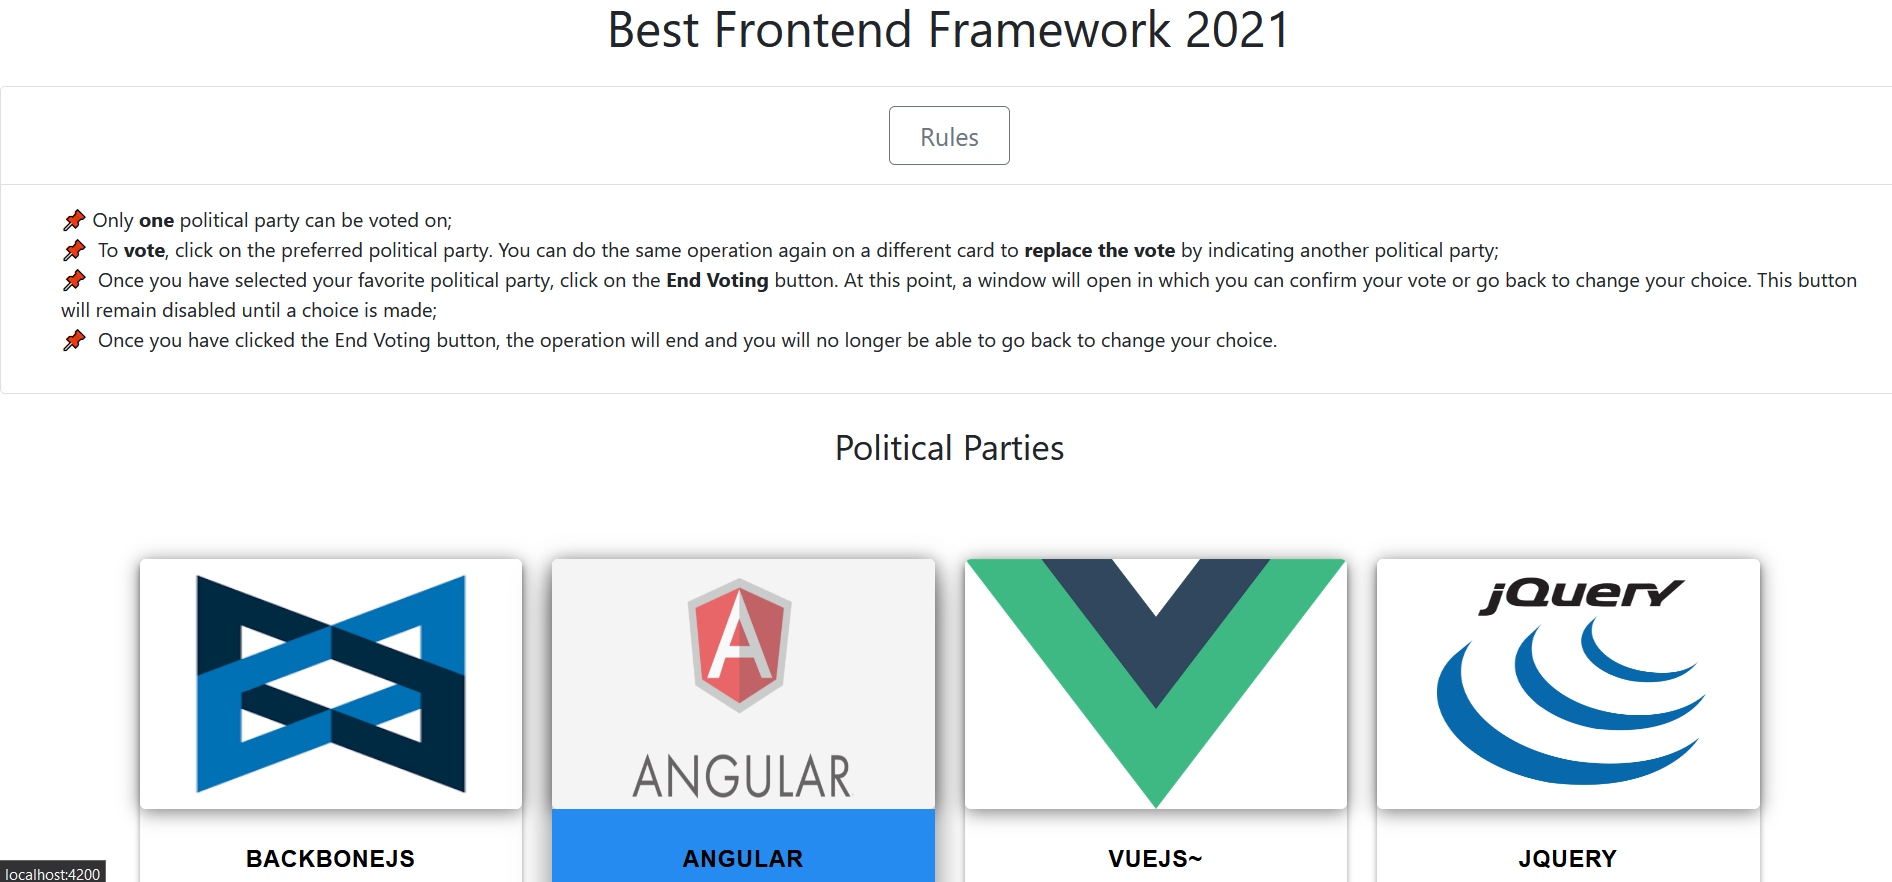
\includegraphics[width=0.6\columnwidth]{cap4/screen/user-election-detail.png} 
    \caption{Maschera di voto di un'elezione}
\end{figure}
\noindent L'elettore, dopo aver effettuato la procedura di autenticazione nel sistema, viene indirizzato alla maschera di voto dell'elezione in questione. In questa pagina l'utente può eseguire diverse operazioni:
\begin{itemize}
    \item visualizzare una lista, che compare cliccando il pulsante "Rules", contenente le \textit{regole} per esprimere correttamente il proprio voto nella piattaforma;
    \item visualizzare l'elenco dei \textit{partiti partecipanti} all'elezione e, cliccando su uno di essi, esprimere la propria preferenza;
    \item \textit{confermare il voto} cliccando sull'apposito pulsante e, una volta letta la finestra che compare in sovrimpressione contenente l'informazione del partito selezionato, premendo il tasto "Confirm".
\end{itemize}
\begin{figure}[H] 
    \centering 
    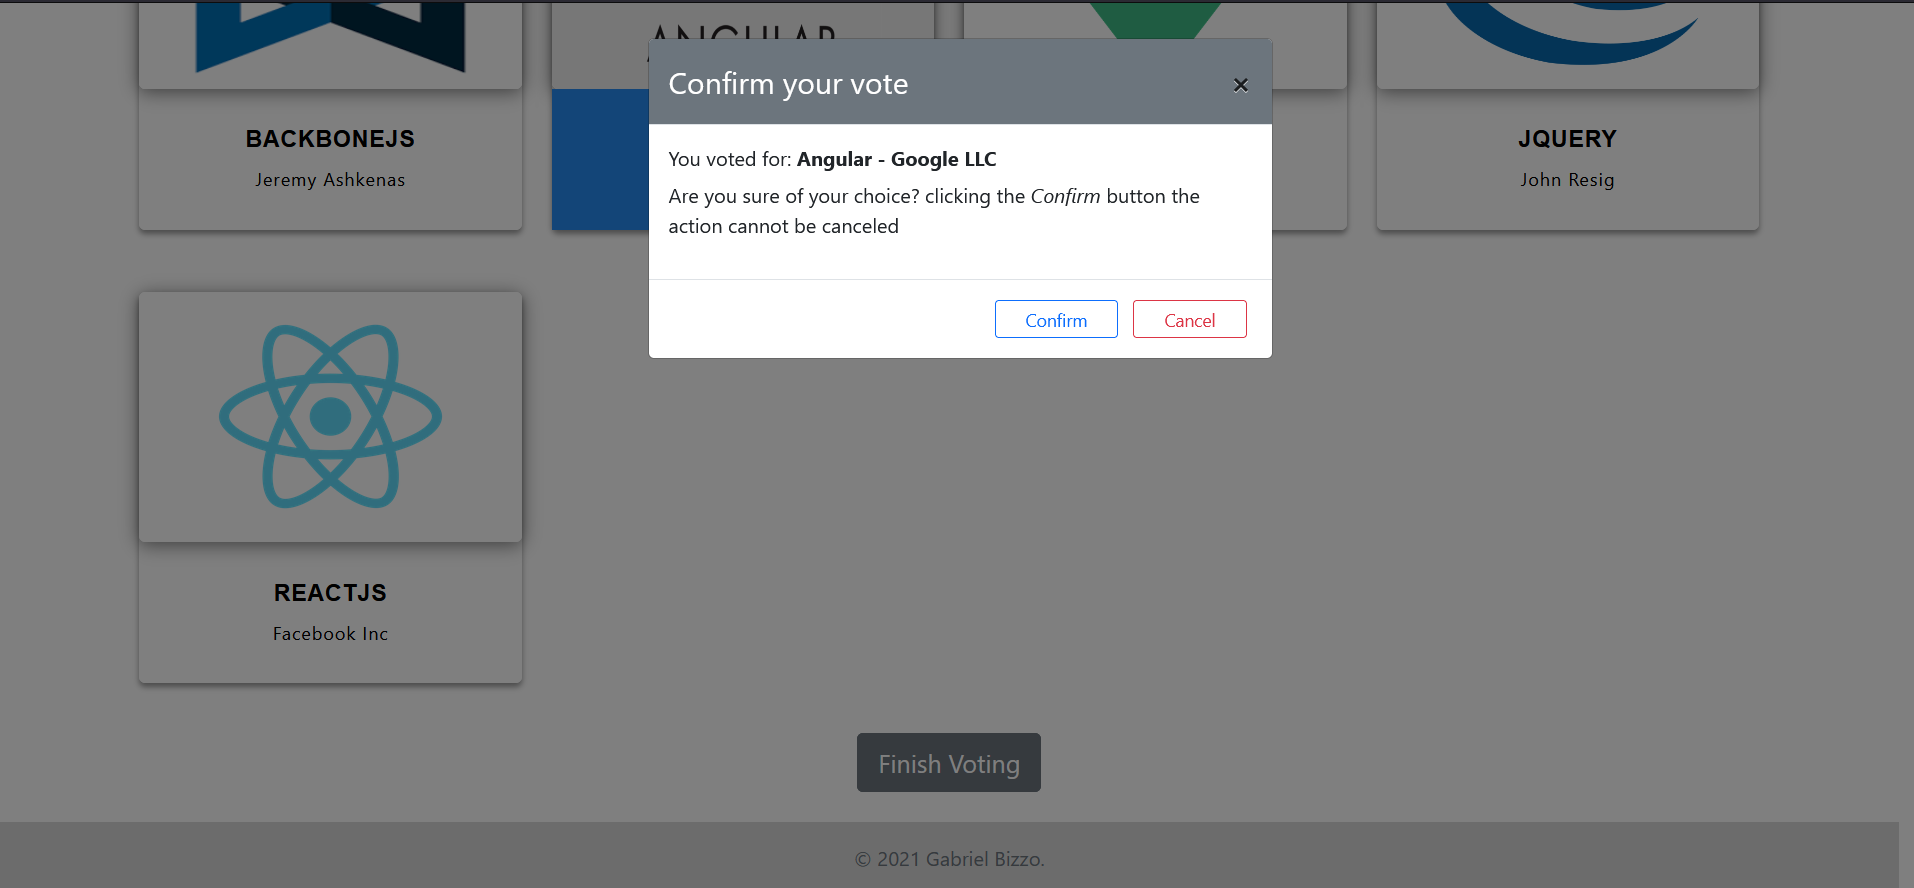
\includegraphics[width=0.6\columnwidth]{cap4/screen/confirm-vote.png} 
    \caption{Pop-up di conferma della preferenza dell'elettore}
\end{figure}
